\documentclass[a4paper]{article}
\usepackage[left=2cm, top=2cm, right=2cm, bottom=3cm]{geometry}
\usepackage[ngerman]{babel}
\usepackage{lmodern}
\usepackage[T1]{fontenc}
\usepackage{graphicx}
\usepackage[pdftitle={Handreichung ArduDigiT}, pdfauthor={Max Kobrow}, pdflang=de-DE]{hyperref}
\usepackage{ccicons}
\renewcommand{\familydefault}{\sfdefault}
\def\CC{{C\nolinebreak[4]\hspace{-.05em}\raisebox{.4ex}{\tiny\bf ++}}}
\usepackage{csquotes}
\MakeOuterQuote{"}
\usepackage{lipsum}
\usepackage{wrapfig}
\usepackage{minted}
\setminted{
    frame=lines,
    framesep=2mm,
    baselinestretch=1.2,
    linenos,
}
\renewcommand{\theFancyVerbLine}{\sffamily {\scriptsize \arabic{FancyVerbLine}}}

\usepackage{enumitem}

\usepackage{parskip}

\begin{document}
\thispagestyle{empty}
\thispdfpagelabel{Titel}
\begin{center}
    \vspace*{5cm}

    \textbf{\Huge Handreichung für Lehrkräfte}

    \vspace*{2cm}

    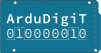
\includegraphics[scale=1]{images/ArduDigiT_Logo_quer_farbig.pdf}

    \vspace*{1cm}

    Letzte Bearbeitung: \today

    \vfill

    Erstellt durch Max Kobrow (\href{mailto:max.kobrow@gmail.com}{max.kobrow@gmail.com}) \\
    Materialien lizenziert unter \href{https://creativecommons.org/licenses/by-sa/4.0/deed.de}{CC BY-SA 4.0 \ccbysa}
\end{center}
\pagebreak
\setcounter{page}{1}

\setcounter{tocdepth}{2}
\tableofcontents

\section{Allgemeines}
\subsection{Zielgruppe}
Der Kurs richtet sich vornehmlich an Schüler*innen des Leistungskurses Informatik an Gymnasien beziehungsweise des Leistungskurses Informatiksysteme an beruflichen Gymnasien in Sachsen. Mögliche Lernbereiche am allgemeinbildenden Gymnasium sind die Lernbereiche 7 \emph{Rechnernetze} und 1 \emph{Technische Informatik}. Am beruflichen Gymnasien wäre ein Einsatz vor allem im Lernbereich 3 \emph{Realisierung von IuK-Systemen in Netzwerken} denkbar.

Der Einsatz in anderen Bundesländern und in Grundkursen ist auch möglich, wird hier aber nicht weiter behandelt.

\subsection{Voraussetzungen}
\subsubsection{Vorwissen}
\begin{itemize}
    \item Programmiererfahrungen, vorzugsweise in einer textuellen Sprache
    \item Wissen über logische Operatoren (fakultativ)
    \item Wissen über Binärzahlen (fakultativ)
\end{itemize}

Je nach Vorwissen lassen sich bestimmte Module des Kurses verkürzen. Geben Sie Ihren Schüler*innen also Hinweise, dass sie bestimmte Inhalte schon kennen und überspringen können.

\subsubsection{Technik}
Die hier beschriebenen Voraussetzungen sind nötig, damit der Kurs so, wie er ist eingesetzt werden kann. Mit selbstständigen Anpassungen kann aber auch andere Hardware eingesetzt werden.
\begin{itemize}
    \item Nötige Hardware (pro Pärchen):
    \begin{itemize}
        \item 2 Arduino Mega mit USB-Kabel
        \item 8 LEDs
        \item 8 Vorwiderstände
        \item ungefähr 20 Jumperkabel M-M
        \item 4 Jumperkabel F-M
        \item 2 Breadboards
        \item 1 I2C LCD mit 2 Zeilen à 16 Zeichen
        \item 2 Knöpfe
    \end{itemize}
    \item installierte Arduino IDE
\end{itemize}

\subsubsection{Moodle}
Geplant ist normalerweise die Verwendung der Moodle-Instanz des Sächsischen Bildungsservers, auf die über \url{schullogin.de} zugegriffen werden kann. Dafür wird dann mittels der Backup-Datei des Kurses dieser als neuer Kurs installiert.

Soll eine eigene Moodle-Instanz verwendet werden, ist das \href{https://docs.moodle.org/402/de/Fragetyp_Coderunner}{Coderunner-Plugin} zwingend notwendig. Außerdem ist es sinnvoll die Filter für die Auto-Verlinkung der \href{https://docs.moodle.org/402/de/Auto-Verlinkung_der_Aktivit%C3%A4tsnamen}{Aktivitätsnamen} und der \href{https://docs.moodle.org/402/de/Auto-Verlinkung_zu_Glossaren}{Glossareinträge} zu aktivieren.

\subsection{Hinweise}
Die ersten drei Module besitzen denselben Aufbau. Sie beginnen mit einem oder mehreren theoretischen Inputs und enden mit einer praktischen Arbeit. Dabei müssen entweder Programmieraufgaben in Moodle erledigt werden (Modul 1 und 3) oder Arduino-Systeme gebaut und programmiert werden (Modul 2 und 4). Außerdem enthält jedes Modul ein Glossar, das wichtige Begriffe des Moduls zusammenfasst und zur Wiederholung verfügbar macht.

Um eine Überforderung der Schüler*innen zu verhindern, werden die Module und Aktivitäten nach und nach freigeschaltet. Das geschieht in den meisten Fällen automatisch, für den Abschluss der Module 2 und 4 mit den Arduino-Aufgaben müssen Sie allerdings tätig werden. Um den Abschluss für Ihre Schüler*innen zu markieren, gehen sie im Kopfbereich des Kurses auf "Bewertungen" (siehe Abbildung \ref{fig:screenshot_bewertungen}). Ist der Bearbeitungsmodus (oben rechts) eingeschaltet, können Sie hier Bewertungen festlegen. Um den Abschluss von Modul 2 zu markieren, tragen Sie in der entsprechenden Zeile in der Spalte \emph{Modul 2 Abschluss} eine 1 ein und drücken Sie auf "Änderungen speichern" (1 steht im Kurs für erledigt/ bestanden, 0 für nicht erledigt/ bestanden). Für Modul 4 ist das Vorgehen analog.

Eine kleine frontale Einführung in den Kurs kann sinnvoll sein, um beispielsweise auf bestimmte Modalitäten bezüglich der Speicherung von Sketches zu geben oder auch um eine Hinführung auf das Thema zu geben.

Zeitlich sind für den Kurs, je nach Vorwissen 3 bis 6 Unterrichtsstunden einzuplanen. Das ist ein sehr großes zeitliches Spektrum, aber der Kurs soll auch ein großes Spektrum an Vorerfahrungen bezüglich Programmierung und Physical Computing abdecken. Die konkrete zeitliche Planung bleibt also Ihnen überlassen.

\begin{figure}[b]
    \centering
    \fbox{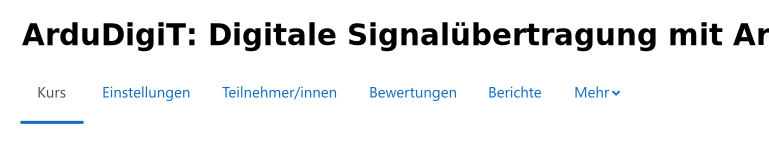
\includegraphics[scale=0.7]{images/screenshot_bewertungen.pdf}}
    \caption{Kopfbereich des Kurses}\label{fig:screenshot_bewertungen}
\end{figure}

\section{Modul 1: Wiederholung Programmierung}
\begin{tabular}{@{}l l}
    \textbf{Abschluss} & automatisch
\end{tabular}
\subsection{Lernziele}
Die Schüler*innen\dots
\begin{itemize}
    \item wiederholen die grundlegenden Programmierkonzepte Variablen, Verzweigungen, Schleifen und Funktionen, indem sie Erklärungen und Beispiele bearbeiten.
    \item kennen die grundlegende Syntax der Arduino-Programmierung (C/ \CC).
    \item kennen mathematische und logische Operatoren, sowie ihre Syntax in der Arduino-Programmierung.
    \item werden sich der syntaktischen Nähe verschiedener Programmiersprachen bewusst.
    \item wenden ihre Kenntnisse an, indem sie eine Lösung implementieren, um gerade Zahlen eines Arrays auf der Konsole auszugeben.
\end{itemize}

\subsection{Elemente}
\subsubsection{Lektion "Crashkurs: imperative Programmierung in C/\CC"}
\begin{minipage}[b][\textheight-1.6cm][t]{0.55\textwidth}
    Die Lektion unterteilt sich in die Bereiche \emph{Einleitung}, \emph{Variablen}, \emph{Verzweigungen}, \emph{Schleifen} und \emph{Funktionen} in denen die jeweiligen Konzepte anhand eines Beispiels erläutert werden. Die einzelnen Seiten und Übergänge sind in der Abbildung rechts detailliert aufgeschlüsselt.

    Die einzelnen inhaltlichen Abschnitte werden jeweils durch Zwischenfragen verbunden, die sichern sollen, dass der vorige Input nachvollzogen wurde. Die Lösungen sind hier kurz aufgeschlüsselt:

    \begin{itemize}
        \item Falsche Zuweisungen
        \begin{itemize}
            \item \mintinline{arduino}|char[] text = "Hallo";| - F
            \item \mintinline{arduino}|int i = 2;| - R
            \item \mintinline{arduino}|bool b = true;| - R
            \item \mintinline{arduino}|int i < 5;| - F
        \end{itemize}
        \item Zuordnung Datentypen
        \begin{itemize}
            \item \mintinline{arduino}|4| - \mintinline{arduino}|int|
            \item \mintinline{arduino}|"Imperative Programmierung"| - \mintinline{arduino}|char| Array
            \item \mintinline{arduino}|'4'| - \mintinline{arduino}|char|
            \item \mintinline{arduino}|true| - \mintinline{arduino}|bool|
        \end{itemize}
        \item Verzweigung Frage 1 und 2
        \begin{itemize}
            \item 10
        \end{itemize}
        \item Schleifen Frage 1
        \begin{itemize}
            \item 10
        \end{itemize}
        \item Schleifen Frage 2
        \begin{itemize}
            \item 5
        \end{itemize}
    \end{itemize}
    
    \subsubsection{Glossar - "Arduino (C/\CC) Syntax - Nachschlagewerk"}
    Das Glossar enthält die Syntax der in der Lektion vorgestellten Inhalte in Kurzform zum Nachschlagen. Einige Befehle, wie \mintinline{c}|printf| werden hier auch tiefer behandelt, als in der Lektion.

    \subsubsection{Quiz - "Bist du bereit?"}
    Diese automatisiert ausgewertete Programmierfrage bildet den Abschluss des Moduls und überprüft, ob die grundlegenden Konzepte der Programmierung und die Arduino-Syntax verstanden wurden. Da es sich nur um ein Modul zur Wiederholung handelt, ist die Aufgabe vergleichsweise einfach gestaltet. Sie soll lediglich alle wichtigen Konstrukte abfragen, aber nicht viel Zeit in Anspruch nehmen.

    Mögliche Lösung:
    \begin{minted}{arduino}
void printEven (int numbers[], int length) {
    for (int i = 0; i < length; i++) {
        if (numbers[i] % 2 == 0) {
            printf("%d ", numbers[i]);
        }
    }
}
    \end{minted}
\end{minipage}\hspace*{5mm}\begin{minipage}[b][\textheight-1.6cm][t]{0.4\textwidth}
    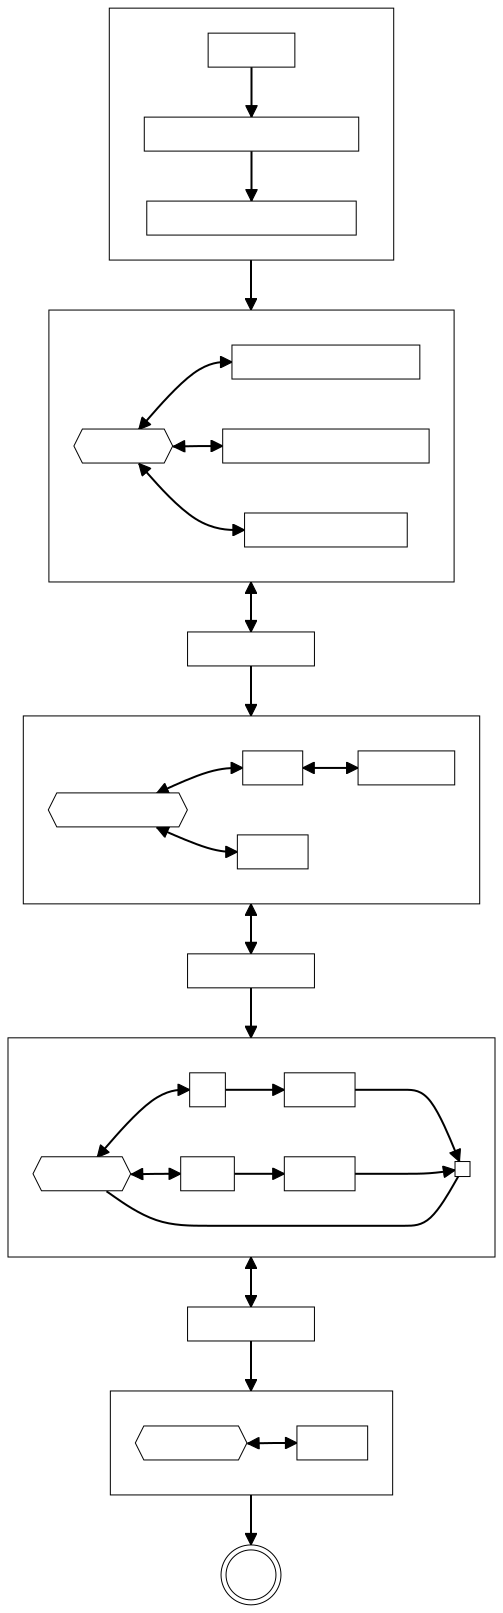
\includegraphics[scale=0.5]{images/programmierung_lektion_flowchart.pdf}
\end{minipage}

\section{Modul 2: Informatisch Basteln mit Arduinos}
\begin{tabular}{@{}l l}
    \textbf{Abschluss} & manuell
\end{tabular}

\subsection{Lernziele}
Die Schüler*innen\dots
\begin{itemize}
    \item kennen spezifische elektrotechnische Bauteile, die für die Bearbeitung des Projekts benötigt werden, vollziehen die Kombination dieser in einem Schaltplan nach und verwenden sie um den Schaltplan nachzubauen.
    \item sind vertraut im Umgang mit der Arduino-IDE und verwenden diese um einen Arduino-Sketch zur Steuerung verschiedener Bauteile mit einem Arduino zu implementieren.
    \item schlagen die Syntax für die Programmierung eigenständig im Kursglossar bzw. in der Arduino-Referenz nach.
\end{itemize}

\subsection{Elemente}
\subsubsection{Buch - "Hardware"}
Diese Inputs behandeln, je nach Gruppe, die relevanten elektronischen Bauteile. Außerdem leiten sie dazu an einen vorgegebenen Bauplan nachzubauen.

\subsubsection{Video - "Tutorial Arduino IDE"}
Diese zwei Videos geben eine kurze Einweisung in die Bedienung der Arduino-IDE. Es gibt zwei Varianten des Videos für die alten Arduino-IDEs mit Version \verb|1.8.*| und die höheren Versionen \verb|2.*|. Je nachdem, welche IDE zum Einsatz kommt, kann die andere Version ausgeblendet werden.

\subsubsection{Buch - "Arduino Programmieren"}
Diese Bücher leiten die Schüler*innen durch die Erstellung des Arduino-Sketches für die Schaltung, die vorher aufgebaut wurde. Sie bieten aber auch die Möglichkeit die Sketche selbstständig zu schreiben und unterstützen dies mit Hilfestellungen.

\subsubsection{Glossar - "Hardware und Arduino-Befehle"}
Hier finden sich die behandelten Befehle speziell zur Steuerung der Hardware übersichtlich wieder.

\section{Modul 3: Wie kommt der Text ins Kabel?}
\begin{tabular}{@{}l l}
    \textbf{Abschluss} & automatisch
\end{tabular}

\subsection{Lernziele}
Die Schüler*innen\dots
\begin{itemize}
    \item unterscheiden zwischen digitaler und analoger Datenübertragung und kennen die Prinzipien der parallelen und seriellen digitalen Datenübertragung.
    \item kennen die Bedeutung von Bit und Byte
    repräsentieren Text mithilfe vom ASCII in Binärdaten.
    \item implementieren die Umwandlung von Text zu Bits und andersherum mithilfe der Arduino-Befehle \mintinline{arduino}|bitRead| und \mintinline{arduino}|bitWrite|.
\end{itemize}

\subsection{Elemente}
\subsubsection{Buch - "Text + Strom = Datenübertragung?"}
Das Buch vermittelt Inhalte zu den Grundlagen der Datenübertragung. Die analoge Übertragung wird kurz angeschnitten, um anschließend näher auf digitale Übertragung und die binäre Codierung von Text einzugehen. Außerdem werden die Arduino-Befehle \mintinline{arduino}|bitRead| und \mintinline{arduino}|bitWrite| eingeführt.

\subsubsection{Glossar - "Befehle und Fakten zur Signalübertragung"}
Hier werden erneut wichtige Befehle und Begriffe des Moduls zusammengefasst.

\subsubsection{Quiz - "bitRead Aufgabe"}
Diese Aufgabe für die Gruppe der Sender beschäftigt sich damit, wie die Bits eines \mintinline{arduino}|char| ausgelesen und ausgegeben werden. Der hier entstandene Code kann später für die Übertragung verwendet werden.

\paragraph{Mögliche Lösung}
\begin{minted}{arduino}
void printBits(char c) {
    for(int i = 7; i >= 0; i--) {
        printf("%d", bitRead(c, i));
    }
}
\end{minted}

\subsubsection{Quiz - "bitWrite Aufgabe"}
Diese Aufgabe ist an die Gruppe der Empfänger gerichtet und beschäftigt sich damit die Bits eines leeren \mintinline{arduino}|char| zu modifizieren, sodass ein Textzeichen dabei herauskommt.

\paragraph{Mögliche Lösung}
\begin{minted}{arduino}
void printChar(int arr[]) {
    char out = '\0';
    for(int i = 0; i < 8; i++) {
        bitWrite(out, 7-i, arr[i]);
    }
    printf("%c", out);
}
\end{minted}


\section{Modul 4: Jetzt bist du dran!}
\begin{tabular}{@{}l l}
    \textbf{Abschluss} & manuell
\end{tabular}

\subsection{Lernziele}
Die Schüler*innen\dots
\begin{itemize}
    \item entwerfen eine Schaltung aus LEDs, Widerständen und einem Arduino, mit dem Daten digital übertragen werden und die Ströme mittels der LEDs sichtbar gemacht werden können. (Sender)
    \item implementieren einen Sketch, der vorgegebenen Text in Binärdaten umwandelt und die GPIO-Ports des Arduino entsprechend der Daten schaltet. (Sender)
    \item entwerfen eine Schaltung aus einem Arduino und einem LCD, mit dem digital übertragene Daten eines Senders empfangen und sichtbar gemacht werden können. (Empfänger)
    \item implementieren einen Sketch, der Text in Form von Binärdaten an den GPIO-Pins des Arduinos empfängt, umwandelt und auf einem LCD ausgibt. (Empfänger)
    \item erkennen Probleme bei der Datenübertragung und diskutieren Lösungen für diese Probleme.
\end{itemize}

\subsection{Mögliche Lösungen}
\paragraph{Sender}
\inputminted{arduino}{code/modul_4_code_sender.ino}

\paragraph{Empfänger}
\inputminted{arduino}{code/modul_4_code_empf.ino}

\subsubsection{Hinweise}
Die Hilfen werden über einen Cookie erst 10 Minuten nachdem die Seite das erste Mal aufgerufen wurde, eingeblendet. Sind Cookies deaktiviert, müssen die Hilfen im HTML Editor bearbeitet werden, damit sie standardmäßig eingeblendet sind.

Die Zusatzaufgaben sollen Schüler*innen, die den Kurs abgeschlossen haben zum Weiterdenken anregen und weitere Themen motivieren. Um mehr Lösungsmöglichkeiten offenzuhalten, wird hier auf Lösungsvorschläge verzichtet. Das gibt Ihnen die Möglichkeit vielleicht auch ohne, dass Sie selbst wissen, wie die Lösung am Ende aussieht, mit Ihren Schüler*innen zu verschiedene Ansätze zu diskutieren.
\end{document}